\documentclass[10pt,twocolumn,letterpaper]{article}

\usepackage[margin=0.72in,columnsep=0.25in]{geometry}
\usepackage{times}
\usepackage[scaled=0.95]{helvet}
\usepackage[T1]{fontenc}
\usepackage{cite}
\usepackage{amsmath,amssymb,amsfonts}
\usepackage{graphicx}
\usepackage{booktabs}
\usepackage{array}
\usepackage{xcolor}
\sloppy

% IEEE Access blue for title, major Roman section headings, and clickable links (no journal logos/headers/footers)
\definecolor{accessblue}{RGB}{0,98,155}

% Balanced two-column float parameters so visuals stay beside their discussing sections
\renewcommand{\topfraction}{0.88}
\renewcommand{\bottomfraction}{0.80}
\renewcommand{\textfraction}{0.10}
\renewcommand{\floatpagefraction}{0.80}
\renewcommand{\dbltopfraction}{0.88}
\renewcommand{\dblfloatpagefraction}{0.80}
\setcounter{topnumber}{3}
\setcounter{bottomnumber}{2}
\setcounter{totalnumber}{4}
\setcounter{dbltopnumber}{2}

\renewcommand{\thesection}{\Roman{section}}
\renewcommand{\thesubsection}{\Alph{subsection}}
\renewcommand{\thetable}{\Roman{table}}

\makeatletter
\renewcommand{\section}{\@startsection{section}{1}{\z@}%
  {-10pt plus -2pt minus -2pt}{4pt plus 1pt}%
  {\normalfont\sffamily\normalsize\bfseries\color{accessblue}\MakeUppercase}}
\renewcommand{\subsection}{\@startsection{subsection}{2}{\z@}%
  {-7pt plus -1pt minus -1pt}{2pt plus 1pt}%
  {\normalfont\normalsize\itshape\color{black}}}
\long\def\@makecaption#1#2{%
  \vskip\abovecaptionskip
  \sbox\@tempboxa{\footnotesize\textbf{\color{accessblue}#1.} #2}%
  \ifdim \wd\@tempboxa >\hsize
    {\footnotesize\textbf{\color{accessblue}#1.} #2\par}
  \else
    \global \@minipagefalse
    \hb@xt@\hsize{\hfil\box\@tempboxa\hfil}%
  \fi
  \vskip\belowcaptionskip}
\makeatother

\usepackage[colorlinks=true,linkcolor=accessblue,citecolor=accessblue,urlcolor=accessblue,bookmarks=true]{hyperref}

\begin{document}

% Clean left-aligned IEEE Access-style title & author typography ONLY (no logo, no running header, no publication footer)
\twocolumn[
\begin{@twocolumnfalse}
\begin{flushleft}
  {\fontsize{19}{22}\selectfont\sffamily\bfseries\color{accessblue} TRUEGUARD: An Empirical Study of White-Box Hallucination Detection, Domain Shift, and Selective Prediction in Large Language Models\par}
  \vspace{8pt}
  {\fontsize{10.5}{13}\selectfont\sffamily\bfseries YOGESH RAVI M\textsuperscript{1}, AND T.\ S.\ PRADEEP KUMAR\textsuperscript{1}, {\normalfont\sffamily\itshape (Senior Member, IEEE)}\par}
  \vspace{3pt}
  {\footnotesize\sffamily\textsuperscript{1}School of Computer Science and Engineering, Vellore Institute of Technology, Chennai, Tamil Nadu, India (e-mail: yogeshravi4343@gmail.com; tspradeepkumar@vit.ac.in)\par}
  \vspace{2pt}
  {\footnotesize\sffamily Corresponding author: T.\ S.\ Pradeep Kumar (e-mail: tspradeepkumar@vit.ac.in).\par}
\end{flushleft}
\vspace{4pt}
\hrule height 0.5pt
\vspace{6pt}
\noindent{\small\textbf{\sffamily\color{accessblue}ABSTRACT}\hspace{0.6em}Large language models frequently produce fluent text that is factually incorrect or unsupported by context. While multi-sample black-box detectors estimate uncertainty by generating repeated answers and scoring them with an auxiliary natural language inference model, single-pass white-box detectors read internal activations, attention weights, and output logits directly. However, their behavior under benchmark artifacts, domain shift, and closed-book selective prediction remains incompletely understood on small frozen models. This paper presents an empirical study of TRUEGUARD, a single-pass white-box framework instrumented on frozen TinyLlama-1.1B-Chat-v1.0 across ten benchmarks (32,590 evaluated sequences). Four internal signal families are combined by logistic regression and paired with a three-tier selective response controller. First, artifact controls show that length and surface-text cues strongly inflate raw HaluEval scores, although white-box probing still outperforms answer-text TF-IDF under strict length matching and is dominated by linear hidden-state probes. Second, zero-shot pooled probes drop to near-chance accuracy on unseen domains, consistent with domain-dependent linear decision boundaries; target-domain few-shot refitting from scratch yields task-dependent gains at 250 labels but trails simple baselines in low-label settings. Third, on closed-book TriviaQA generations, TRUEGUARD trained on 250 target-domain calibration labels outperforms label-free Semantic Entropy and token uncertainty baselines and performs competitively with label-free SelfCheckGPT-NLI, whereas pure selective abstention accounts for the error reduction with no measurable net benefit from active resampling or retrieval.\par}
\vspace{5pt}
\noindent{\small\textbf{\sffamily\color{accessblue}INDEX TERMS}\hspace{0.6em}Abstention, dataset artifacts, domain shift, few-shot refitting, hallucination detection, internal representations, large language models, selective prediction, white-box probing.\par}
\vspace{6pt}
\hrule height 0.5pt
\vspace{9pt}
\end{@twocolumnfalse}
]

% ==============================================================================
\section{Introduction}
\label{sec:introduction}

\subsection{Background and Motivation}
Large language models (LLMs) are now used across question answering, summarization, dialogue, and decision support. Even when their writing appears clear and well structured, these models regularly produce hallucinations, meaning outputs that contradict factual knowledge, invent unsupported details, or depart from the provided source text \cite{review35,review18}. Because fabricated answers often resemble correct ones in tone and grammar, users cannot easily tell when a response is reliable. That uncertainty directly weakens human trust in language model outputs \cite{review19,review03}.

Detecting incorrect answers at inference time is particularly difficult when applications rely on small, frozen open-weight models for privacy, memory, or latency reasons. Several established black-box detectors, including SelfCheckGPT \cite{review21} and Semantic Entropy \cite{kuhn2023semantic,farquhar2024detecting}, sample multiple stochastic responses for each prompt and compare them using an external natural language inference (NLI) model. Although black-box methods require no access to internal model weights, generating many responses per query increases computational work and requires serving a second neural model. White-box methods offer a single-pass alternative. By inspecting hidden activations, attention weights, and token probability distributions during one forward pass, a lightweight classifier can estimate hallucination risk without modifying the frozen language model or generating extra candidate answers \cite{review27,review01,review12}.

\subsection{Problem Statement and Research Gap}
Despite encouraging in-domain results reported in the white-box probing literature, three practical issues complicate real-world use. First, standard hallucination benchmarks such as HaluEval \cite{review29} pair human or reference answers with synthetically generated hallucinations. High accuracy on those benchmarks may reflect differences in answer length or writing style rather than genuine detection of factual errors. Second, supervised probes trained on one group of benchmarks often lose accuracy when applied to a new domain. Practitioners therefore need to know whether small amounts of target-domain labeled data can restore performance, and whether refitted white-box probes actually outperform simpler one-dimensional or text-only baselines. Third, when a detector is connected to a response controller that can resample, retrieve external evidence, or abstain, evaluation must separate the accuracy gained by abstaining on risky questions from the net effect of active correction attempts.

Previous studies have investigated linear hidden-state probing \cite{review27,review28}, attention patterns \cite{review09,review11}, token entropy and energy \cite{review04,review17}, multi-sample black-box consistency \cite{review21}, and retrieval-based revision \cite{review25,review33}. However, these components are usually studied in separate setups or without joint artifact and baseline controls. Little empirical evidence examines all four internal signal families inside one frozen small model across ten datasets while simultaneously quantifying length and TF-IDF benchmark artifacts, comparing within-domain and cross-domain probe directions at equal sample sizes, benchmarking target-only few-shot refitting against simple baselines, and auditing abstention versus active multi-tier intervention alongside reproduced external baselines on the same closed-book generations.

\subsection{Research Objectives and Main Contributions}
This study evaluates TRUEGUARD on frozen \texttt{TinyLlama/TinyLlama-1.1B-Chat-v1.0} to answer four research questions: (1) how much in-domain white-box detection survives length and TF-IDF artifact controls; (2) why pooled white-box probes fail under zero-shot domain shift; (3) when target-domain few-shot refitting from scratch ($K \in \{50, 100, 250\}$) outperforms source-risk recalibration and simple baselines; and (4) how target-refitted single-pass detection compares with label-free multi-sample external baselines on TriviaQA, and whether active resampling or retrieval improves upon pure selective abstention.

Rather than claiming individual white-box signals or selective routing as new algorithmic inventions, this work uses TRUEGUARD as a unified experimental framework and makes three evidence-backed empirical contributions. First, across five in-domain benchmarks (18,141 rows), we show that headline HaluEval AUROCs (0.9880 QA, 0.9936 Summarization) are heavily inflated by length (0.9572 on HaluEval-QA) and answer-text TF-IDF (0.9661 QA, 0.9539 Summarization); yet TRUEGUARD significantly beats answer-text TF-IDF on all four paired benchmarks under strict length matching ($|\Delta L| \le 2$; +0.0331 to +0.0829 AUROC, $p \le 0.035$), while ISP carries over 96\% of the fusion weight. Second, across four unseen benchmarks (13,949 rows), pooled zero-shot probes collapse to chance (0.4597 to 0.5205) and source-risk recalibration fails (0.4957 to 0.5242); equal-sample-size diagnostics ($N = 900$) show higher within-domain (+0.1125 to +0.6707) than cross-domain (-0.0151 to +0.0204) probe alignment, while target-only few-shot refitting ($K = 250$, under 2~s CPU) yields task-dependent gains on FaithDial (0.8231), FEVER (0.7325), and WikiBio (0.6698), ties 1D length on XSum (0.6456 vs.\ 0.6445), and trails simpler baselines at $K = 50$. Third, on 250 held-out closed-book TriviaQA generations, target-refitted single-pass TRUEGUARD ($K = 250$; 0.7876 AUROC, 0.4360 AURC) significantly outperforms label-free 10-sample Semantic Entropy (0.6859, $p_{\text{Holm}} = 0.012$), Predictive Entropy (0.6583, $p_{\text{Holm}} = 0.006$), and verified length-normalized NLL (0.4678, $p_{\text{Holm}} = 0.006$), and performs competitively with label-free 10-sample SelfCheckGPT-NLI (0.7477, $p_{\text{Holm}} = 0.478$, n.s.), whereas zero-shot pooled TRUEGUARD scores 0.5504. Forensically, pure selective abstention at 46.0\% coverage (64/115 correct, 55.65\%) drives error reduction, while the full three-tier controller (63/115, 54.78\%; four fixed, three broken) shows no measurable net benefit from active interventions.

Section~\ref{sec:related} reviews related work, Section~\ref{sec:framework} details TRUEGUARD, Section~\ref{sec:methodology} presents experimental protocols, Section~\ref{sec:results} reports results, Section~\ref{sec:discussion} discusses implications and limitations, and Section~\ref{sec:conclusion} concludes.

% ==============================================================================
\section{Related Work}
\label{sec:related}

\subsection{Hallucinations and Internal-State Detection}
Surveys divide hallucinations into intrinsic errors contradicting source text and extrinsic errors introducing unverifiable claims \cite{review35,review18}. Evaluations confirm frequent factual errors in closed-book QA, biographies, and dialogue \cite{review37,review23}, motivating benchmarks such as TruthfulQA \cite{review22}, HaluEval \cite{review29}, and self-contradiction suites \cite{review36}, alongside studies linking unreliability to human trust \cite{review03,review19}. Internal-state detectors test whether frozen activations separate truthful from fabricated text. Azaria and Mitchell \cite{review27} introduced SAPLMA to probe intermediate hidden layers, followed by unsupervised monitoring in MIND \cite{review01}, prompt-guided probing in PRISM \cite{review02}, deep representation analysis \cite{review05}, representation-shift tracking in HalluShift \cite{review13}, single-pass semantic-entropy probes \cite{review14}, and activation steering in ITI \cite{review28} and Truth Forest \cite{review38}.

\subsection{Attention, Uncertainty, Domain Shift, and Mitigation}
Attention and uncertainty studies include LLM-Check \cite{review12}, attention-pattern tracing \cite{review09}, uncertainty-aware heads \cite{review11}, predictive entropy surveys \cite{review07}, token entropy production rates \cite{review17}, and semantic energy \cite{review04}. Black-box multi-sample baselines such as SelfCheckGPT \cite{review21} and Semantic Entropy \cite{kuhn2023semantic,farquhar2024detecting} draw multiple responses and score consistency via NLI. Because synthetic benchmarks like HaluEval \cite{review29} can introduce length or stylistic artifacts, evaluating probes without text-only controls and cross-domain splits risks overstating generalization. For mitigation, active approaches include RAG \cite{review25}, Self-RAG \cite{review26}, Chain-of-Verification \cite{review24}, RARR \cite{review33}, FacTool \cite{review34}, CRITIC \cite{review39}, multi-agent debate \cite{review31}, and calibrated reinforcement learning \cite{review15}. When active correction is unreliable, selective prediction and risk-coverage analysis (AURC) \cite{geifman2017selective} trade coverage for lower error rates. TRUEGUARD combines four established internal signal families into one frozen-model testbed to jointly evaluate artifact sensitivity, cross-domain failure, target-only refitting, external baselines, and selective abstention.

% Place Figure 1 right before Section III so it lands at top of the Section III page
\begin{figure*}[!t]
\centering
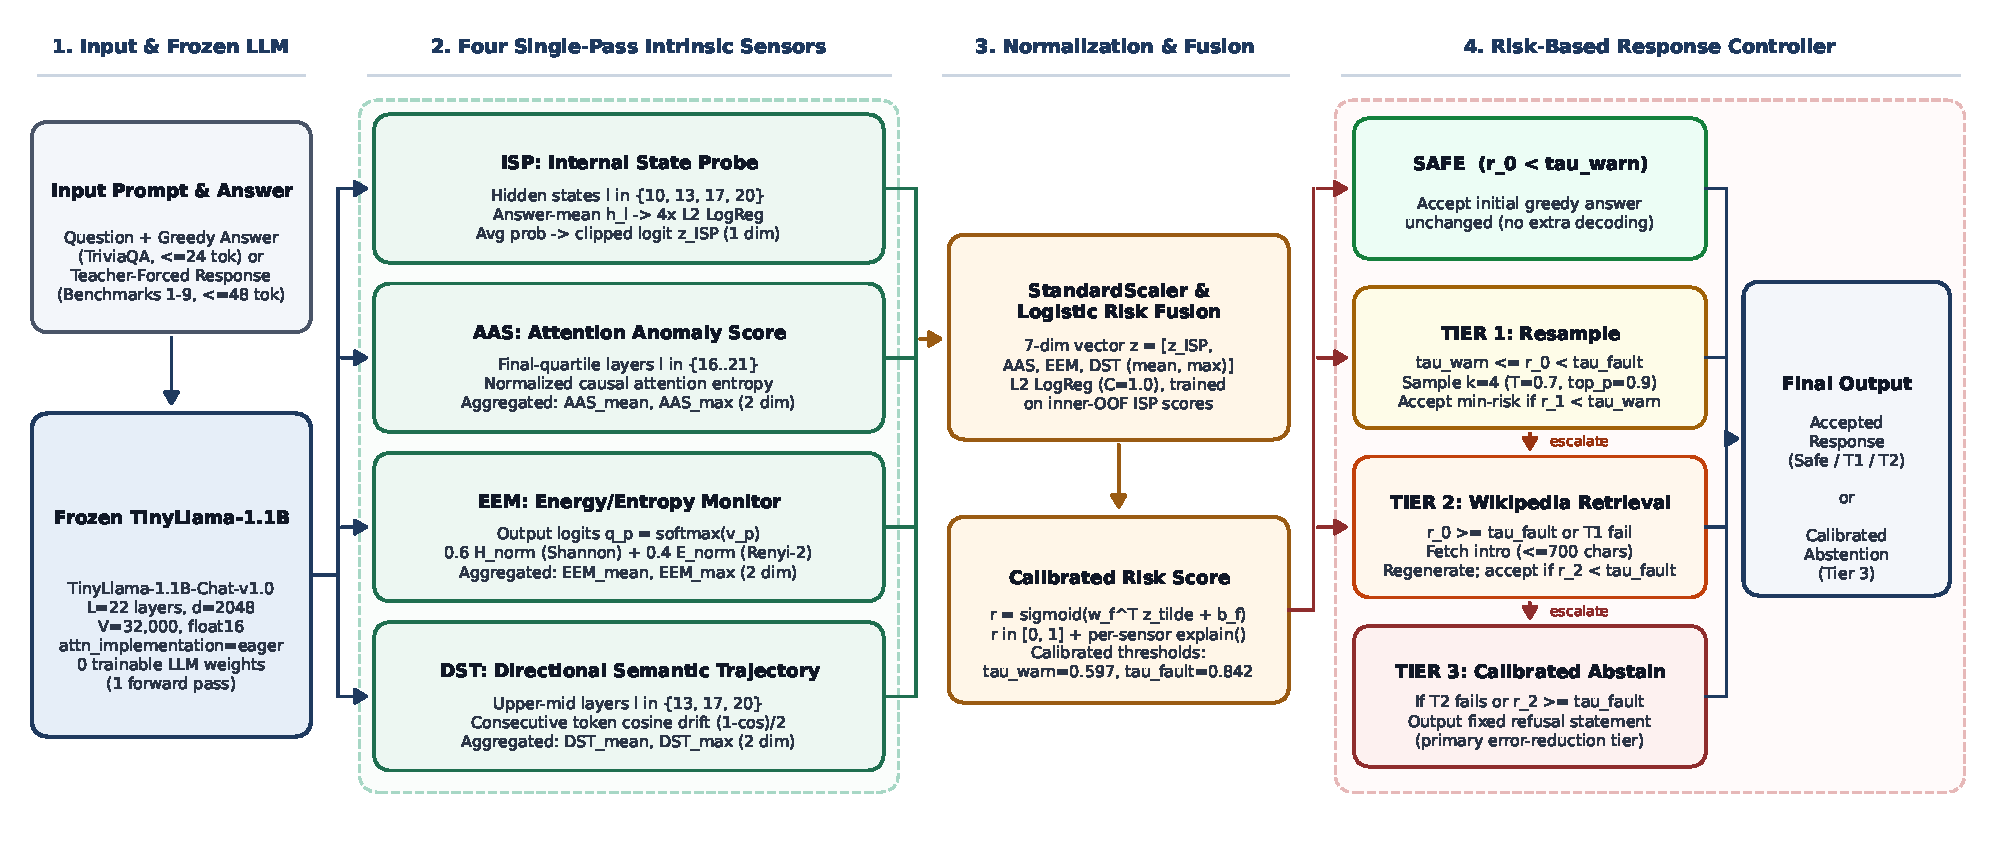
\includegraphics[width=\textwidth]{figures/Fig1_TRUEGUARD_Architecture.pdf}
\caption{Overview of the TRUEGUARD single-pass white-box framework attached to frozen TinyLlama-1.1B-Chat-v1.0. Four intrinsic signal families (ISP, AAS, EEM, DST) are extracted in parallel in one forward pass, normalized and fused by an L2-regularized logistic classifier into a calibrated hallucination risk score $r \in [0, 1]$, and routed through a three-tier selective response controller (SAFE, TIER 1 Resample, TIER 2 Wikipedia Retrieval, TIER 3 Calibrated Abstain). Conceptual diagram matching \texttt{tg\_pipeline.py} and \texttt{tg\_controller.py}.}
\label{fig:arch}
\end{figure*}

% ==============================================================================
\section{Proposed TRUEGUARD Framework}
\label{sec:framework}

\subsection{System Architecture and Foundation Model}
TRUEGUARD attaches a white-box monitor and selective controller to frozen \texttt{TinyLlama/TinyLlama-1.1B-Chat-v1.0} \cite{zhang2024tinyllama} without modifying any base LLM weights ($L = 22$ decoder layers, $N_h = 23$ hidden-state tensors including embeddings, hidden dimension $d = 2048$, vocabulary $V = 32{,}000$, \texttt{float16} on CUDA, \texttt{attn\_implementation="eager"}). As shown in Fig.~\ref{fig:arch}, TRUEGUARD runs in three stages: single-pass extraction of four intrinsic signal families, regularized logistic risk fusion, and threshold-governed response routing. Two mathematically equivalent extraction paths are implemented and unit-tested: teacher-forced scoring (\texttt{score\_answer}, truncated to 384 prompt and 48 answer tokens) and token-by-token cached monitoring (\texttt{OnlineSignalMonitor}, 24 maximum new tokens on TriviaQA).

\subsection{Internal State Probe (ISP)}
Following multi-layer linear probing \cite{review27}, hidden states are extracted at depth fractions $\mathcal{F}_{\text{ISP}} = \{0.45, 0.60, 0.75, 0.90\}$, corresponding to layer indices $\mathcal{L}_{\text{ISP}} = \{10, 13, 17, 20\}$. For an answer spanning token positions $[a_{\text{start}}, a_{\text{end}})$ of length $T_a = a_{\text{end}} - a_{\text{start}}$, each probed layer's states predicting answer tokens are mean-pooled:
\begin{equation}
\bar{h}_l = \frac{1}{T_a} \sum_{p = a_{\text{start}} - 1}^{a_{\text{end}} - 2} h_{l,p} \in \mathbb{R}^{d}, \qquad l \in \mathcal{L}_{\text{ISP}},
\label{eq:isp_mean}
\end{equation}
where $h_{l,p} \in \mathbb{R}^{d}$ is the hidden-state vector at layer $l$ and position $p$. Each layer's standardized vector $\tilde{h}_l$ feeds an L2-regularized logistic regression classifier $(w_l, b_l)$ with $C \in \{0.001, 0.01, 0.1\}$ chosen via inner 5-fold group-preserving CV maximizing AUROC. Layer probabilities are averaged and mapped to clipped log-odds:
\begin{equation}
p_{\text{ISP}} = \frac{1}{|\mathcal{L}_{\text{ISP}}|} \sum_{l \in \mathcal{L}_{\text{ISP}}} \sigma\!\left(w_l^\top \tilde{h}_l + b_l\right), \quad z_{\text{ISP}} = \log\!\left(\frac{\tilde{p}}{1 - \tilde{p}}\right),
\label{eq:isp_prob}
\end{equation}
where $\sigma(x) = (1 + e^{-x})^{-1}$, $|\mathcal{L}_{\text{ISP}}| = 4$, and $\tilde{p} = \text{clip}(p_{\text{ISP}}, 10^{-4}, 1 - 10^{-4})$.

\subsection{Attention Anomaly Score (AAS)}
AAS measures causal attention dispersion across final-quartile layers $\mathcal{L}_{\text{AAS}} = \{\lfloor 0.75 L \rfloor, \dots, L - 1\}$ (layers 16--21). Letting $a_{l,h,p,j} \in [0, 1]$ denote the attention weight of head $h \in \{1, \dots, H\}$ in layer $l$ from query $p$ to key $j \le p + 1$, normalized Shannon entropy is averaged across heads and layers:
\begin{equation}
\text{AAS}_p = \frac{1}{|\mathcal{L}_{\text{AAS}}|\, H} \sum_{l \in \mathcal{L}_{\text{AAS}}} \sum_{h=1}^{H} \frac{-\sum_{j=1}^{p+1} a_{l,h,p,j} \log\!\left(a_{l,h,p,j} + \epsilon\right)}{\max(\log(p+1),\, 1)},
\label{eq:aas}
\end{equation}
with $\epsilon = 10^{-10}$, aggregated as $\text{AAS}_{\text{mean}}$ and $\text{AAS}_{\text{max}}$.

\subsection{Energy/Entropy Monitor (EEM)}
From raw output logits $v_p \in \mathbb{R}^{V}$ and $q_p = \text{softmax}(v_p)$, EEM computes normalized Shannon entropy and normalized R\'enyi-2 collision entropy:
\begin{equation}
\begin{aligned}
H_{\text{norm}}(q_p) &= \text{clip}\!\left(\frac{-\sum_{i=1}^{V} q_{p,i} \log(q_{p,i} + \epsilon)}{\log V},\, 0,\, 1\right), \\
E_{\text{norm}}(q_p) &= \text{clip}\!\left(\frac{-\log\!\left(\sum_{i=1}^{V} q_{p,i}^2 + \epsilon\right)}{\log V},\, 0,\, 1\right),
\end{aligned}
\label{eq:eem_parts}
\end{equation}
combined with fixed weight $w_e = 0.6$:
\begin{equation}
\text{EEM}_p = w_e\, H_{\text{norm}}(q_p) + (1 - w_e)\, E_{\text{norm}}(q_p),
\label{eq:eem}
\end{equation}
and summarized as $\text{EEM}_{\text{mean}}$ and $\text{EEM}_{\text{max}}$. Standalone predictive entropy ($\text{ENT}_{\text{mean}}$), length-normalized NLL, and token length (LEN) are logged strictly as baselines and never fused.

\subsection{Directional Semantic Trajectory (DST)}
DST tracks step-to-step representational drift across consecutive answer tokens using the layer-averaged hidden state $u_p = \frac{1}{|\mathcal{L}_{\text{DST}}|} \sum_{l \in \mathcal{L}_{\text{DST}}} h_{l,p}$ over $\mathcal{L}_{\text{DST}} = \{13, 17, 20\}$:
\begin{equation}
\text{DST}_p = \text{clip}\!\left(\frac{1 - \cos(u_p, u_{p-1})}{2},\, 0,\, 1\right),
\label{eq:dst}
\end{equation}
for $p \ge a_{\text{start}}$ (undefined for the first token; defaulting to $0.0$ for one-token answers), aggregated as $\text{DST}_{\text{mean}}$ and $\text{DST}_{\text{max}}$.

% Place Table I just before Section IV so it lands at the top of the Section IV page
\begin{table*}[!t]
\centering
\caption{Ten-Dataset Benchmark Suite, Protocol Roles, Splits, and Exclusions}
\label{tab:datasets}
\resizebox{\textwidth}{!}{%
\begin{tabular}{cllrrrrrrc}
\toprule
\# & Dataset & Protocol Role & Raw Rows & Usable Rows & Groups & Label 0 & Label 1 & Prevalence & Excluded \\
\midrule
1 & \texttt{halueval\_dialogue} & \texttt{IN\_DOMAIN\_CV\_AND\_POOL} & 10,000 & 4,000 & 2,000 & 2,000 & 2,000 & 0.500 & 0 \\
2 & \texttt{halueval\_qa} & \texttt{IN\_DOMAIN\_CV\_AND\_POOL} & 10,000 & 4,000 & 2,000 & 2,000 & 2,000 & 0.500 & 0 \\
3 & \texttt{halueval\_summarization} & \texttt{IN\_DOMAIN\_CV\_AND\_POOL} & 10,000 & 4,000 & 2,000 & 2,000 & 2,000 & 0.500 & 0 \\
4 & \texttt{truthful\_qa} & \texttt{IN\_DOMAIN\_CV\_AND\_POOL} & 817 & 1,634 & 817 & 817 & 817 & 0.500 & 0 \\
5 & \texttt{halueval\_general} & \texttt{IN\_DOMAIN\_CV\_AND\_POOL} & 4,507 & 4,507 & 4,507 & 3,692 & 815 & 0.181 & 0 \\
6 & \texttt{faithdial} & \texttt{UNSEEN\_ZEROSHOT\_AND\_TARGET\_REFIT} & 3,539 & 3,507 & 791 & 946 & 2,561 & 0.730 & 32 \\
7 & \texttt{wikibio\_gpt3} & \texttt{UNSEEN\_ZEROSHOT\_AND\_TARGET\_REFIT} & 1,908 & 1,908 & 238 & 516 & 1,392 & 0.730 & 0 \\
8 & \texttt{xsum\_factuality} & \texttt{UNSEEN\_ZEROSHOT\_AND\_TARGET\_REFIT} & 5,597 & 1,868 & 498 & 185 & 1,683 & 0.901 & 1 \\
9 & \texttt{fever} & \texttt{UNSEEN\_CLAIM\_VERIFICATION\_REFIT} & 18,999 & 6,666 & 6,666 & 3,333 & 3,333 & 0.500 & 12,333 \\
10 & \texttt{trivia\_qa} & \texttt{CLOSED\_BOOK\_SELECTIVE\_PREDICTION} & 17,944 & 250 cal + 250 test & 500 & Dynamic & Dynamic & 0.660 (test) & 0 \\
\bottomrule
\end{tabular}}
\end{table*}

\subsection{Risk Fusion Classifier and Three-Tier Controller}
The four sensors form a standardized 7-dimensional vector $\tilde{z}$ mapped to calibrated risk $r \in [0, 1]$ by L2 logistic regression ($C_{\text{fusion}} = 1.0$):
\begin{equation}
\begin{aligned}
z &= \big[z_{\text{ISP}},\; \text{AAS}_{\text{mean}},\; \text{AAS}_{\text{max}},\; \text{EEM}_{\text{mean}},\; \text{EEM}_{\text{max}},\; \text{DST}_{\text{mean}},\; \text{DST}_{\text{max}}\big]^\top, \\
r &= \sigma\!\left(w_{\text{f}}^\top \tilde{z} + b_{\text{f}}\right),
\end{aligned}
\label{eq:fusion}
\end{equation}
where $w_{\text{f}} \in \mathbb{R}^7$ and $b_{\text{f}} \in \mathbb{R}$ are fitted strictly on inner out-of-fold ISP probabilities to prevent probe-to-fusion leakage before refitting layer probes on the full training fold. For closed-book generation, \texttt{ThreeTierController} routes an initial greedy answer $a_0$ (risk $r_0$) using calibration-selected thresholds $\tau_w < \tau_f$ ($\tau_w = \tau_{\text{warning}}$, $\tau_f = \tau_{\text{fault}}$):
\begin{equation}
\small
g(r_0) = \begin{cases}
\text{SAFE (accept } a_0\text{)}, & r_0 < \tau_w, \\
\text{T1 (sample } k{=}4\text{; } r_1{<}\tau_w\text{)}, & \tau_w \le r_0 < \tau_f, \\
\text{T2 (Wiki } {\le}700\text{ ch; } r_2{<}\tau_f\text{)}, & r_0 \ge \tau_f \text{ or T1 fail}, \\
\text{T3 (calibrated abstain)}, & \text{T2 fail or } r_2 \ge \tau_f,
\end{cases}
\label{eq:controller}
\end{equation}
where Tier 1 draws $k = 4$ stochastic candidates ($T = 0.7$, $\text{top\_p} = 0.9$, 24 tokens), Tier 2 prepends an introductory Wikipedia extract via \texttt{WikipediaRetriever}, and Tier 3 outputs a fixed refusal. Monitoring alone requires one LLM forward pass and zero auxiliary NLI models.

% ==============================================================================
\section{Experimental Methodology}
\label{sec:methodology}

\begin{figure*}[!t]
\centering
\includegraphics[width=\textwidth]{figures/Fig_Section4_Experimental_Protocol.pdf}
\caption{Three-track experimental protocol, data separation, and statistical validation across all ten benchmarks (Table~\ref{tab:datasets}). Track~1 evaluates in-domain 5-fold \texttt{GroupKFold} CV alongside four CPU-only artifact controls; Track~2 transfers the pooled source model zero-shot to unseen domains before diagnostic checks and target-only refitting from scratch on 60\%/40\% group-disjoint splits; Track~3 evaluates closed-book TriviaQA generations while separating supervised calibration from label-free ranking baselines (all GPU runs on Colab NVIDIA T4, 16~GB VRAM, \texttt{seed = 42}; sequential latency profiled on 25 prompts $\times$ 24 forced tokens, \texttt{eager}, \texttt{batch\_size = 1}).}
\label{fig:protocol}
\end{figure*}

As shown in Fig.~\ref{fig:protocol}, our evaluation covers ten public benchmarks totaling 32,590 sequences (Table~\ref{tab:datasets}) across three tracks: five in-domain datasets totaling 18,141 examples from HaluEval \cite{review29} and TruthfulQA \cite{review22} under 5-fold \texttt{GroupKFold} CV with zero group overlap; four initially unseen datasets---FaithDial \cite{dziri2022faithdial}, WikiBio-GPT3 \cite{review21}, XSum-Factuality \cite{maynez2020faithfulness}, and FEVER \cite{thorne2018fever} (reported separately for claim-verification transfer, excluding 12,333 \texttt{NOT ENOUGH INFO} items)---for zero-shot and target-only refitting; and closed-book TriviaQA \cite{joshi2017triviaqa} (250 calibration and 250 disjoint test questions; $y = 1$ when greedy generation fails to match an accepted answer alias). Datasets 1--9 use teacher-forced scoring (\texttt{seed = 42}; zero \texttt{NaN}/\texttt{Inf} values), and token-length-normalized NLL is computed identically across all ten datasets:
\begin{equation}
\text{NLL} = \frac{1}{T_a} \sum_{t = a_{\text{start}}}^{a_{\text{end}} - 1} \left(-\log \text{softmax}(v_{t-1})_{x_t}\right),
\label{eq:nll}
\end{equation}
where $x_t$ is the target token at position $t$ and $v_{t-1}$ is its predicting logit vector. On Track~1, the four CPU-only artifact controls use identical 5-fold splits: answer length (LEN), answer-text TF-IDF (word 1--2 and character \texttt{char\_wb} 3--5 grams, 15,000 features each, zero LLM or prompt access), shuffled-label leakage checks, and length-matched pairs ($|\Delta L| \le 2$ tokens; paired group-level bootstrap 95\% CIs, $B = 1{,}000$). On Track~2, cross-domain diagnostics compare within-domain split-half against cross-domain probe-weight cosines on full datasets and at equal sample size ($N_{\text{fit}} = 900$ per half, 3 seeds $\times$ 4 layers, vs.\ 2,048-d random null $0.0000 \pm 0.0221$) alongside within-length-quartile and length-matched EEM AUROCs; target-only refitting trains fresh probes from scratch (zero source weight transfer) on $K \in \{50, 100, 250\}$ grouped examples from 60\% pools across ten seeds (0--9) and tests on fixed 40\% group-disjoint splits against Source Risk Recalibration (SrcRecal), 1D EEM, 1D LEN, and TF-IDF on identical $K$ examples (using exact Colab \texttt{.npz} zero-shot baselines to avoid 0.0005--0.0081 local \texttt{scikit-learn 1.3.2} unpickling drift; because Datasets 6--9 were inspected during zero-shot diagnosis, these 40\% splits measure target-only sample efficiency rather than independent external confirmation, with repeated-seed SDs holding the test split fixed \cite{nadeau2003inference}). On Track~3, target-refitted TRUEGUARD fits probes, fusion, and thresholds ($\tau_w = 0.5973$, $\tau_f = 0.8415$) from scratch on the 250 labeled calibration generations with zero test-label access, while unchanged \texttt{TRUEGUARD\_Pooled\_ZS} uses zero target labels; in contrast, reproduced SelfCheckGPT-NLI \cite{review21} (\texttt{potsawee/\allowbreak deberta-v3-large-mnli}, \texttt{float16}, $M = 10$, $T = 0.7$, $\text{top\_p} = 0.9$, single-sentence short-answer scoring), Semantic Entropy \cite{kuhn2023semantic,farquhar2024detecting} (\texttt{microsoft/\allowbreak deberta-large-mnli}, \texttt{float32}, $M = 10$, relaxed bidirectional entailment, both length-normalized and discrete variants), Predictive Entropy, and NLL rank risk completely label-free, using calibration labels only for Youden's J binary F1 cutoffs. In-domain 95\% CIs use 500 group-level bootstraps, while TriviaQA 95\% CIs and paired two-sided $p$-values use $B = 1{,}000$ paired bootstraps with the finite-sample bound:
\begin{equation}
p_{\text{boot}} = \frac{1 + 2 \min(n_{\le 0},\, n_{\ge 0})}{B + 1},
\label{eq:pboot}
\end{equation}
Holm--Bonferroni adjusted across six head-to-head TriviaQA comparisons ($p_{\text{Holm}} \ge 0.0060$); an independent zero-import audit verified all saved metrics to $1.11 \times 10^{-16}$.

% Place Table II just before Section V-A so it lands right on the Section V-A page
\begin{table*}[!t]
\centering
\caption{In-Domain 5-Fold Group-Preserving Cross-Validation With Dataset-Artifact Controls (LM: Length-Matched $|\Delta L|\le 2$ Tokens)}
\label{tab:indomain}
\resizebox{\textwidth}{!}{%
\begin{tabular}{lrcccccccccc}
\toprule
Dataset & Rows & TG AUROC [95\% CI] & ISP & ECE & LEN CV & TF-IDF & Shuf. & LM $n$ (\%) & LM: TG [95\% CI] & LM: TF-IDF [95\% CI] & LM: $\Delta$ ($p_{\text{boot}}$) \\
\midrule
\texttt{halueval\_dialogue} & 4,000 & \textbf{0.9218} [0.915, 0.929] & 0.9221 & 0.0220 & 0.7087 & 0.8618 & 0.5072 & 1,352 (33.8\%) & \textbf{0.7996} [0.782, 0.818] & 0.7167 [0.697, 0.737] & \textbf{+0.0829} (0.0010) \\
\texttt{halueval\_qa} & 4,000 & \textbf{0.9880} [0.984, 0.991] & 0.9880 & 0.0095 & \textbf{0.9572} & \textbf{0.9661} & 0.4894 & 256 (6.4\%) & \textbf{0.7901} [0.744, 0.837] & 0.7440 [0.693, 0.794] & \textbf{+0.0461} (0.0350) \\
\texttt{halueval\_summarization} & 4,000 & \textbf{0.9936} [0.992, 0.995] & 0.9936 & 0.0099 & 0.4902 & \textbf{0.9539} & 0.4971 & 3,546 (88.6\%) & \textbf{0.9939} [0.992, 0.995] & 0.9608 [0.955, 0.966] & \textbf{+0.0331} (0.0010) \\
\texttt{truthful\_qa} & 1,634 & \textbf{0.8773} [0.861, 0.894] & 0.8772 & 0.0251 & 0.5510 & 0.8064 & 0.4928 & 714 (43.7\%) & \textbf{0.8106} [0.782, 0.840] & 0.7394 [0.707, 0.772] & \textbf{+0.0712} (0.0010) \\
\texttt{halueval\_general} & 4,507 & \textbf{0.7204} [0.702, 0.740] & 0.7225 & 0.0055 & 0.5089 & 0.6944 & 0.5123 & N/A & N/A & N/A & N/A \\
\bottomrule
\end{tabular}}
\end{table*}

% ==============================================================================
\section{Results and Analysis}
\label{sec:results}

\subsection{In-Domain Detection, Artifact Controls, and Sensor Ablation}
Table~\ref{tab:indomain} reports 5-fold group CV and dataset-artifact controls across Datasets 1--5. TRUEGUARD achieves 0.9218 AUROC on HaluEval-Dialogue, 0.9880 on HaluEval-QA, 0.9936 on HaluEval-Summarization, 0.8773 on TruthfulQA, and 0.7204 on imbalanced HaluEval-General (0.3868 AUPRC, 2.1 times random baseline), with low calibration error (ECE 0.0055--0.0251). However, artifact controls reveal strong surface confounds in HaluEval: on HaluEval-QA, 1D answer length alone reaches 0.9572 AUROC and answer-text TF-IDF reaches 0.9661, with only 6.4\% of pairs (128 pairs) matching within two tokens; on that length-matched subset (where raw length drops to 0.5516), TRUEGUARD drops 19.8 points to 0.7901. On HaluEval-Summarization, length is neutral (0.4902), but answer-text TF-IDF reaches 0.9539 (0.9608 length-matched), reflecting synthetic style cues. High raw HaluEval AUROCs therefore do not alone establish generalizable factual error detection.

Even so, real above-surface signal survives. Shuffled-label AUROCs remain at chance (0.4894--0.5123). TRUEGUARD beats answer-text TF-IDF on all five full benchmarks (+0.0219 to +0.0709) and significantly outperforms TF-IDF on all four length-matched paired subsets ($|\Delta L| \le 2$): +0.0829 on HaluEval-Dialogue ($p = 0.0010$), +0.0461 on HaluEval-QA ($p = 0.0350$), +0.0331 on HaluEval-Summarization ($p = 0.0010$), and +0.0712 on TruthfulQA ($p = 0.0010$), with similar margins when TF-IDF is refitted strictly inside each length-matched subset (0.7072, 0.7322, 0.9586, 0.7501). Other subtler dataset artifacts may still remain.

Leave-one-sensor-out ablations across all five in-domain datasets establish that ISP dominates fusion: removing ISP drops AUROC by -0.0584 (HaluEval-QA) to -0.2709 (HaluEval-Summarization), whereas removing AAS, EEM, or DST alters AUROC by at most 0.0018 (ISP-only matches 4-sensor fusion within $\pm 0.0021$). In the pooled source fusion model, standardized \texttt{ISP\_logit} carries weight +2.9353 (over 96\% of total weight magnitude vs.\ $|w| \le 0.0680$ for all six scalar features). Four-sensor fusion thus does not consistently outperform ISP alone in AUROC; auxiliary sensors contribute primarily via low-FPR unique detections (raising HaluEval-General union Recall@10\% FPR from 0.348 to 0.529, +18.1\%) and low-label fallbacks under domain shift.

% Table III & Figure 2 paired cleanly for Section V-B
\begin{table*}[!t]
\centering
\caption{Target-Domain Few-Shot Refitting (Target-Only Probe Training) vs.\ Source Recalibration and Simple Baselines (ZS: Zero-Shot)}
\label{tab:fewshot}
\resizebox{\textwidth}{!}{%
\begin{tabular}{lcccccccc}
\toprule
Target Dataset (40\% Test) & ZS Exact & $K$ & Target-Only TG (10 seeds) & Source Risk Recal. & 1D EEM Cal. & 1D Length (LEN) & Answer TF-IDF & $K{=}250$ ECE (ZS) \\
\midrule
\texttt{faithdial} & 0.4929 & 50 & 0.6987 $\pm$ 0.0881 & 0.4957 $\pm$ 0.0060 & \textbf{0.7473} $\pm$ 0.0000 & 0.6721 $\pm$ 0.0000 & 0.5818 $\pm$ 0.0406 & N/A \\
\texttt{faithdial} & 0.4929 & 100 & \textbf{0.7899} $\pm$ 0.0313 & 0.5029 $\pm$ 0.0069 & 0.7473 $\pm$ 0.0000 & 0.6721 $\pm$ 0.0000 & 0.6145 $\pm$ 0.0249 & N/A \\
\texttt{faithdial} & 0.4929 & 250 & \textbf{0.8231} $\pm$ 0.0121 & 0.5043 $\pm$ 0.0060 & 0.7473 $\pm$ 0.0000 & 0.6721 $\pm$ 0.0000 & 0.6615 $\pm$ 0.0187 & \textbf{0.0443} (0.6574) \\
\midrule
\texttt{wikibio\_gpt3} & 0.4883 & 50 & 0.5088 $\pm$ 0.0562 & 0.4977 $\pm$ 0.0121 & 0.5000 $\pm$ 0.0235 & 0.4909 $\pm$ 0.0470 & \textbf{0.5321} $\pm$ 0.0274 & N/A \\
\texttt{wikibio\_gpt3} & 0.4883 & 100 & 0.4939 $\pm$ 0.0840 & 0.4977 $\pm$ 0.0121 & 0.5045 $\pm$ 0.0231 & 0.4727 $\pm$ 0.0384 & \textbf{0.5785} $\pm$ 0.0395 & N/A \\
\texttt{wikibio\_gpt3} & 0.4883 & 250 & \textbf{0.6698} $\pm$ 0.0381 & 0.5023 $\pm$ 0.0121 & 0.4955 $\pm$ 0.0231 & 0.4909 $\pm$ 0.0470 & 0.6103 $\pm$ 0.0290 & \textbf{0.0737} (0.4336) \\
\midrule
\texttt{xsum\_factuality} & 0.4597 & 50 & 0.5401 $\pm$ 0.0686 & 0.5000 $\pm$ 0.0425 & \textbf{0.6082} $\pm$ 0.0855 & 0.5867 $\pm$ 0.1218 & 0.5329 $\pm$ 0.0457 & N/A \\
\texttt{xsum\_factuality} & 0.4597 & 100 & 0.6058 $\pm$ 0.0430 & 0.5242 $\pm$ 0.0340 & 0.6352 $\pm$ 0.0000 & \textbf{0.6445} $\pm$ 0.0000 & 0.5331 $\pm$ 0.0370 & N/A \\
\texttt{xsum\_factuality} & 0.4597 & 250 & \textbf{0.6456} $\pm$ 0.0410 & 0.5161 $\pm$ 0.0389 & 0.6352 $\pm$ 0.0000 & \textbf{0.6445} $\pm$ 0.0000 & 0.5456 $\pm$ 0.0323 & \textbf{0.0383} (0.5629) \\
\midrule
\texttt{fever} (claim verif.) & 0.5205 & 50 & 0.5394 $\pm$ 0.0482 & 0.5123 $\pm$ 0.0173 & 0.5176 $\pm$ 0.0425 & 0.4977 $\pm$ 0.0117 & \textbf{0.5699} $\pm$ 0.0183 & N/A \\
\texttt{fever} (claim verif.) & 0.5205 & 100 & \textbf{0.6195} $\pm$ 0.0395 & 0.5000 $\pm$ 0.0216 & 0.5264 $\pm$ 0.0371 & 0.4955 $\pm$ 0.0110 & 0.5966 $\pm$ 0.0224 & N/A \\
\texttt{fever} (claim verif.) & 0.5205 & 250 & \textbf{0.7325} $\pm$ 0.0136 & 0.5000 $\pm$ 0.0216 & 0.5264 $\pm$ 0.0371 & 0.5045 $\pm$ 0.0110 & 0.6315 $\pm$ 0.0104 & \textbf{0.0430} (0.3419) \\
\bottomrule
\end{tabular}}
\end{table*}

\begin{figure*}[!t]
\centering
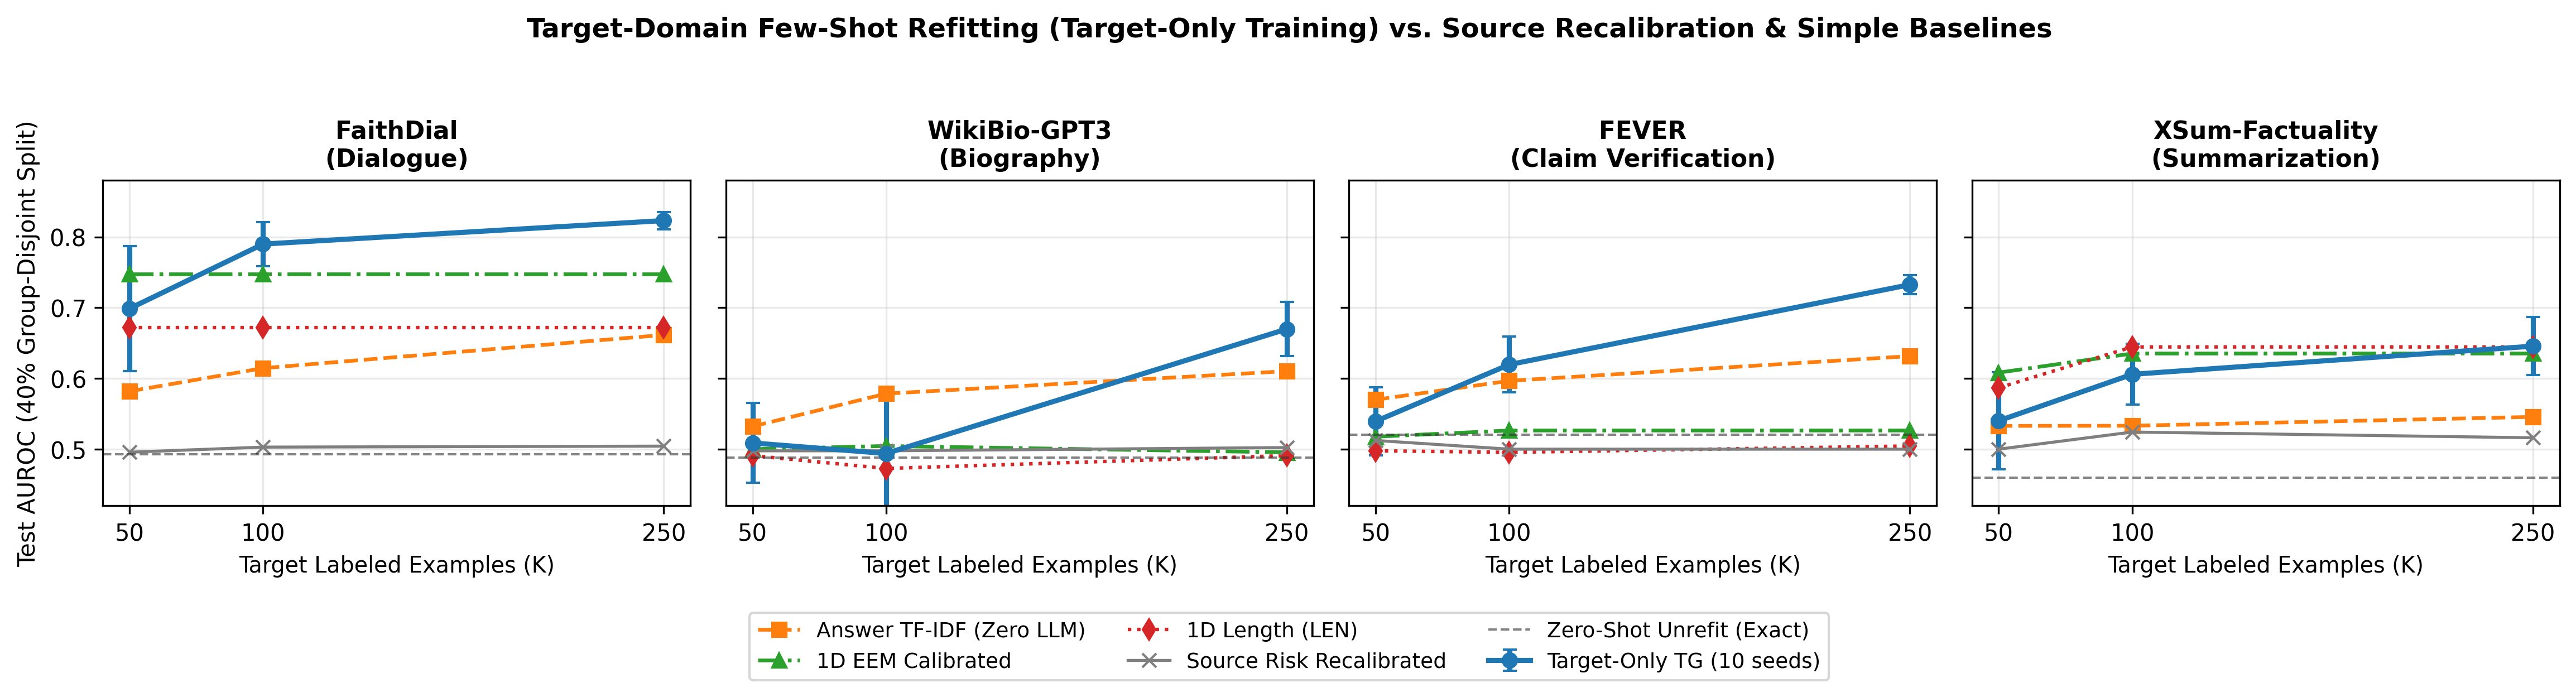
\includegraphics[width=\textwidth]{figures/Fig2_TargetDomain_FewShot_Refitting_vs_Baselines.png}
\caption{Target-domain few-shot refitting ($K = 50, 100, 250$, 10 seeds) compared with zero-shot unrefitted TRUEGUARD, source risk recalibration, 1D EEM, 1D LEN, and answer-text TF-IDF across four group-disjoint 40\% test sets.}
\label{fig:fewshot}
\end{figure*}

\subsection{Zero-Shot Collapse and Target-Domain Few-Shot Refitting}
Pooled zero-shot transfer collapses to near-chance across all four unseen benchmarks (exact Colab \texttt{.npz} 40\% test AUROCs: FaithDial 0.4929, WikiBio-GPT3 0.4883, XSum-Factuality 0.4597, FEVER 0.5205; ECE 0.3419--0.6574), even though target 5-fold ISP AUROC reaches 0.8927 (FaithDial), 0.8754 (FEVER), 0.7427 (WikiBio), and 0.6794 (XSum). Table~\ref{tab:fewshot} and Fig.~\ref{fig:fewshot} show Target-Domain Few-Shot Refitting (target-only training, zero source weights transferred). Source Risk Recalibration remains at chance (0.4957--0.5242). At $K = 50$, simple baselines beat 2,048-dimensional TRUEGUARD probes on every dataset (1D EEM leads FaithDial 0.7473 and XSum 0.6082; TF-IDF leads WikiBio 0.5321 and FEVER 0.5699). At $K = 250$ (under 2~s CPU), gains are task-dependent: TRUEGUARD clearly beats all simple baselines on FaithDial (0.8231), FEVER (0.7325), and WikiBio (0.6698) and cuts ECE by 82\%--93\%, whereas on XSum-Factuality it approximately matches 1D length (0.6456 vs.\ 0.6445).

% Table IV & Figure 3 paired cleanly for Section V-C
\begin{table*}[!t]
\centering
\caption{Empirical Domain-Shift Diagnostics: Within-Domain vs.\ Cross-Domain Probe Alignment and Length-Controlled EEM}
\label{tab:diag}
\resizebox{\textwidth}{!}{%
\begin{tabular}{lccccccc}
\toprule
Dataset & Within-Domain Cos (Full) & Within-Domain Cos ($N{=}900$) & Cross-Domain Cos (Pool / $N{=}900$) & Raw $\text{EEM}_{\text{mean}}$ & $\rho(\text{EEM}, \text{LEN})$ & Quartile Mean EEM & LM ($|\Delta L|\le 2$) EEM \\
\midrule
\texttt{halueval\_summarization} & +0.6888 $\pm$ 0.0132 & +0.6707 $\pm$ 0.0129 & Source & 0.5787 & -0.0658 & 0.5331 & 0.5770 \\
\texttt{halueval\_qa} & +0.4358 $\pm$ 0.0246 & +0.4999 $\pm$ 0.0363 & Source & \textbf{0.3627} & \textbf{-0.2909} & 0.4465 & \textbf{0.5184} \\
\texttt{halueval\_dialogue} & +0.3929 $\pm$ 0.0379 & +0.3930 $\pm$ 0.0280 & Source & \textbf{0.3740} & -0.1038 & \textbf{0.3795} & \textbf{0.4525} \\
\texttt{truthful\_qa} & +0.3440 $\pm$ 0.0269 & N/A & Source & 0.4912 & -0.3678 & 0.4720 & 0.5030 \\
\texttt{halueval\_general} & +0.0506 $\pm$ 0.0252 & N/A & Source & 0.4829 & -0.1637 & 0.4545 & N/A \\
\texttt{fever} & +0.3680 $\pm$ 0.0212 & +0.2668 $\pm$ 0.0189 & +0.0510 / +0.0204 & 0.5417 & -0.4285 & 0.5547 & N/A \\
\texttt{faithdial} & +0.2300 $\pm$ 0.0206 & +0.2205 $\pm$ 0.0168 & -0.0306 / -0.0151 & \textbf{0.7456} & \textbf{+0.0058} & \textbf{0.7662} & N/A \\
\texttt{wikibio\_gpt3} & +0.1290 $\pm$ 0.0224 & +0.1282 $\pm$ 0.0318 & -0.0045 / +0.0032 & 0.5207 & -0.2348 & 0.5278 & N/A \\
\texttt{xsum\_factuality} & +0.1073 $\pm$ 0.0272 & +0.1125 $\pm$ 0.0295 & +0.0280 / +0.0092 & \textbf{0.6648} & \textbf{-0.0321} & \textbf{0.6648} & N/A \\
\midrule
\textit{Random 2048-d Null} & \textit{0.0000 $\pm$ 0.0221} & \textit{0.0000 $\pm$ 0.0221} & \textit{0.0000 $\pm$ 0.0221} & \textit{0.5000} & \textit{0.0000} & \textit{0.5000} & \textit{0.5000} \\
\bottomrule
\end{tabular}}
\end{table*}

\begin{figure*}[!t]
\centering
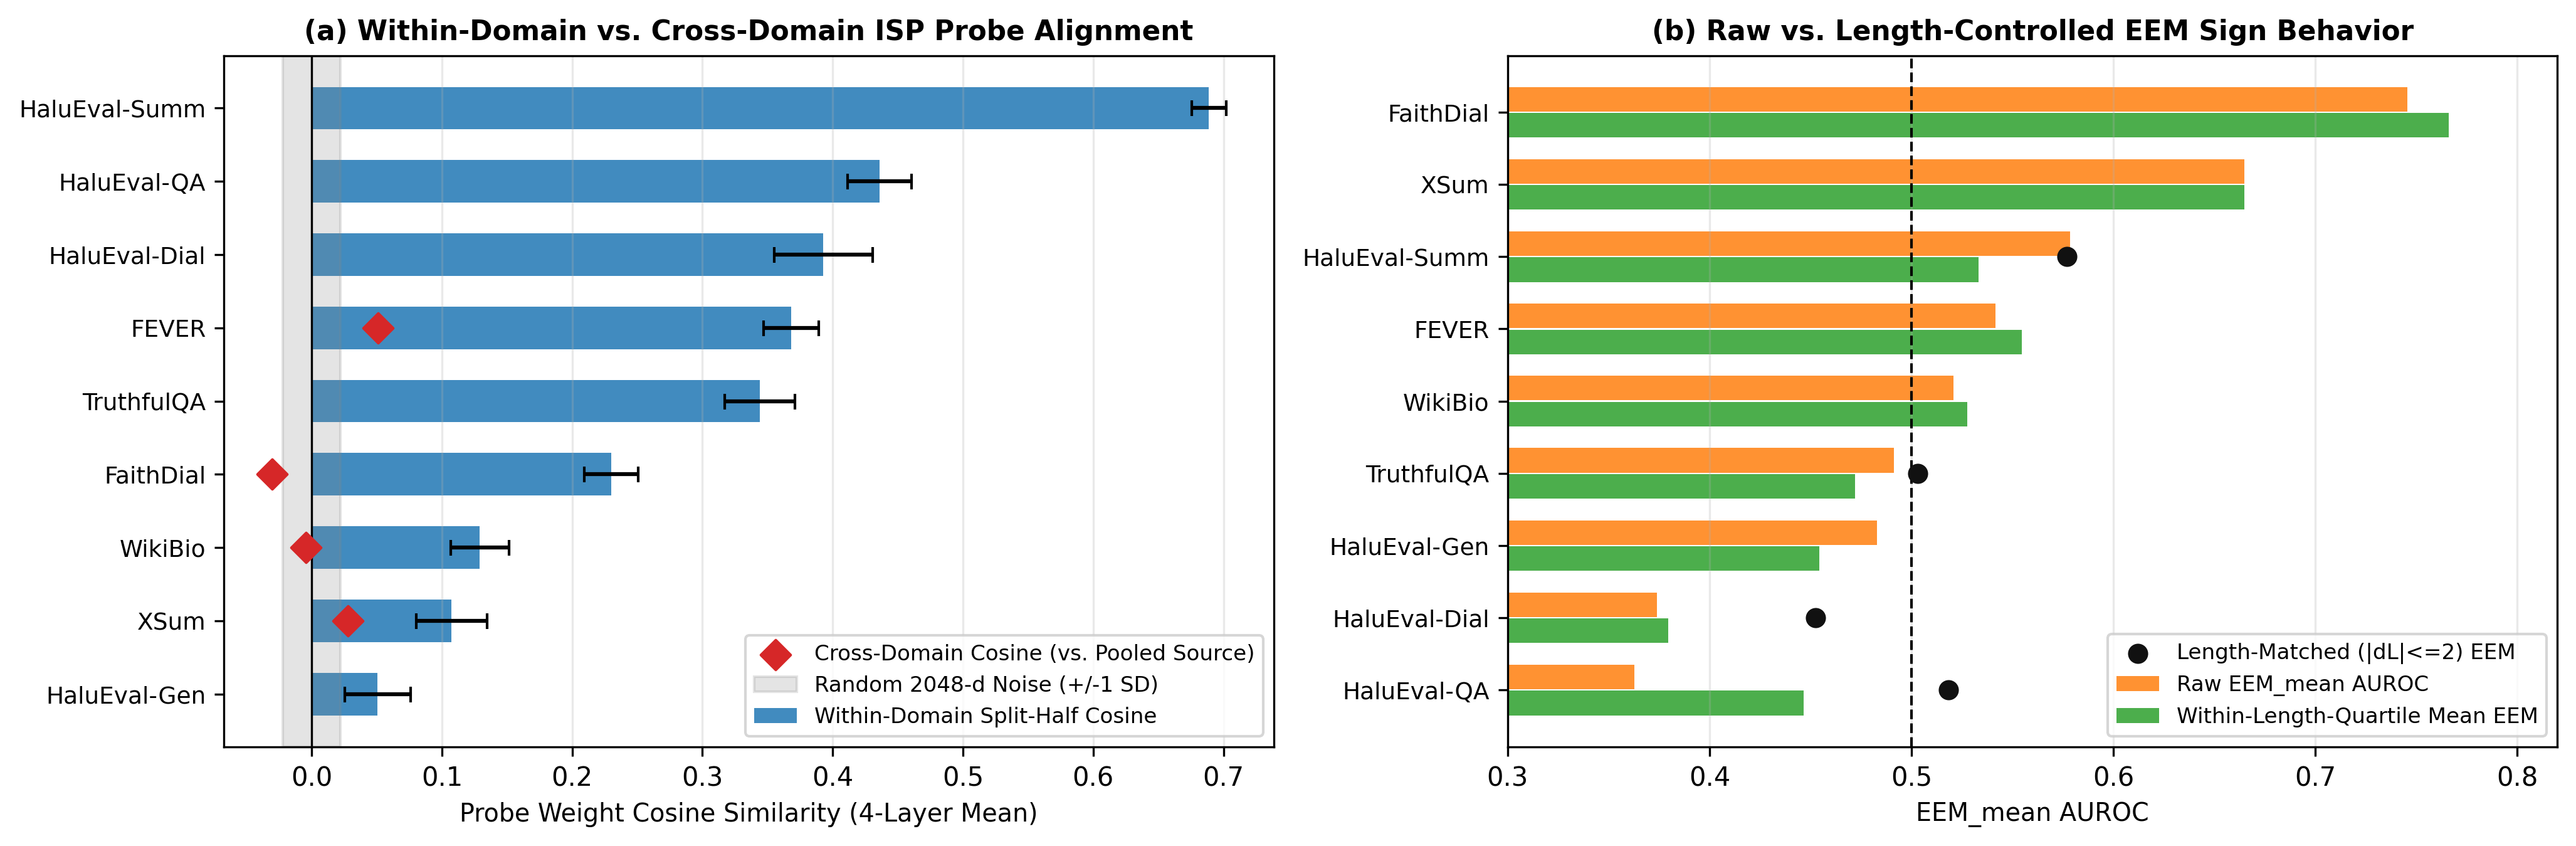
\includegraphics[width=\textwidth]{figures/Fig8_CrossDomain_Diagnostics_Cosine_and_LengthControlled_EEM.png}
\caption{Empirical domain-shift diagnostics: (a) within-domain split-half vs.\ cross-domain ISP probe weight cosine similarity relative to the 2,048-d random noise band; (b) raw vs.\ length-controlled $\text{EEM}_{\text{mean}}$ AUROC across nine benchmarks.}
\label{fig:diag}
\end{figure*}

\subsection{Cross-Domain Probe Alignment and Length-Controlled Entropy}
Table~\ref{tab:diag} and Fig.~\ref{fig:diag} summarize our domain-shift diagnostics. Against the 2,048-d random null ($0.0000 \pm 0.0221$), within-domain split-half probe weight cosines reach +0.2300 to +0.6888 on homogeneous benchmarks (10--31 times random SD), whereas cross-domain cosines against pooled source probes lie between -0.0306 and +0.0510. At strictly equal sample size ($N_{\text{fit}} = 900$ per half), within-domain cosines remain +0.1125 (XSum) to +0.6707 (HaluEval-Summ), while cross-domain cosines stay near zero (-0.0151 to +0.0204). Because L2 coefficients in correlated high-dimensional spaces are not unique causal directions, we interpret this contrast strictly as empirical diagnostic evidence consistent with domain-dependent linear decision boundaries.

Length-controlled EEM analysis (Table~\ref{tab:diag}, Fig.~\ref{fig:diag}(b)) separates three regimes: on FaithDial ($\rho = +0.0058$, quartile-mean 0.7662) and XSum ($\rho = -0.0321$, quartile-mean 0.6648), positive EEM signal persists unchanged after length control; on HaluEval-QA ($\rho = -0.2909$), length matching eliminates the raw inversion (0.3627 to 0.5184); and on HaluEval-Dialogue, the inverse association persists within length quartiles (0.3795) and partially under length matching (0.4525).

% Table V & Figure 4 for Section V-D (External Baselines)
\begin{table*}[!t]
\centering
\caption{Head-to-Head Comparison Against External Baselines on Identical 250 TriviaQA Test Questions (Supervision-Distinguished)}
\label{tab:external}
\resizebox{\textwidth}{!}{%
\begin{tabular}{llclccccccc}
\toprule
Method ($n_{\text{cal}}{=}250, n_{\text{test}}{=}250$) & Supervision / Target Labels & Gens/Q & Extra Model & AUROC [95\% CI] & AUPRC & F1 (Cal) & AURC [95\% CI] & Acc@46\% & $\Delta$AUROC ($p_{\text{Holm}}$) & $\Delta$AURC ($p_{\text{Holm}}$) \\
\midrule
\textbf{TRUEGUARD\_4sensor} & Supervised (250 cal) & 1 & None & \textbf{0.7876} [0.720, 0.852] & 0.8460 & \textbf{0.8084} & \textbf{0.4360} [0.360, 0.523] & \textbf{55.6\%} & N/A & N/A \\
\textbf{TRUEGUARD\_ISP\_only} & Supervised (250 cal) & 1 & None & 0.7706 [0.701, 0.834] & 0.8476 & 0.8062 & 0.4473 [0.369, 0.532] & 53.9\% & +0.0170 (0.478) & -0.0113 (0.451) \\
\textbf{TRUEGUARD\_Pooled\_ZS} & Zero-Shot (0 target) & 1 & None & 0.5504 & 0.7124 & N/A & 0.6342 & 37.4\% & +0.2372 & -0.1982 \\
\textbf{SelfCheckGPT\_NLI} & Label-Free (0 rank; 250 thr) & 11 & DeBERTa-v3-L & 0.7477 [0.681, 0.812] & \textbf{0.8537} & 0.5920 & 0.4659 [0.385, 0.559] & 50.4\% & +0.0399 (0.478) & -0.0299 (0.362) \\
\textbf{Semantic\_Entropy\_LN} & Label-Free (0 rank; 250 thr) & 10 & DeBERTa-L & 0.6859 [0.621, 0.756] & 0.8059 & 0.6377 & 0.5411 [0.450, 0.627] & 49.6\% & \textbf{+0.1017 (0.012)} & \textbf{-0.1051 (0.006)} \\
\textbf{Semantic\_Entropy\_Disc} & Label-Free (0 rank; 250 thr) & 10 & DeBERTa-L & 0.6856 [0.620, 0.753] & 0.8025 & 0.6403 & 0.5414 [0.452, 0.629] & 48.7\% & \textbf{+0.1020 (0.012)} & \textbf{-0.1054 (0.006)} \\
\textbf{Predictive\_Entropy} & Label-Free (0 rank; 250 thr) & 1 & None & 0.6583 [0.587, 0.730] & 0.7471 & 0.5985 & 0.5309 [0.448, 0.617] & 45.2\% & \textbf{+0.1293 (0.006)} & \textbf{-0.0949 (0.006)} \\
\textbf{NLL (Length-Norm.)} & Label-Free (0 rank; 250 thr) & 1 & None & 0.4678 [0.396, 0.542] & 0.6453 & 0.5423 & 0.6843 [0.603, 0.760] & 31.3\% & \textbf{+0.3198 (0.006)} & \textbf{-0.2483 (0.006)} \\
\bottomrule
\end{tabular}}
\end{table*}

\subsection{External Baselines, Selective Abstention, and Efficiency}
On 250 held-out TriviaQA generations (Table~\ref{tab:external}, Fig.~\ref{fig:external}), target-refitted single-pass \texttt{TRUEGUARD\_4sensor} ($K = 250$) reaches 0.7876 AUROC and 0.4360 AURC, significantly outperforming label-free 10-sample Semantic Entropy (0.6859 LN / 0.6856 Disc, $p_{\text{Holm}} = 0.012$; AURC 0.5411, $p_{\text{Holm}} = 0.006$), Predictive Entropy (0.6583, $p_{\text{Holm}} = 0.006$), and NLL (0.4678, $p_{\text{Holm}} = 0.006$), and performing competitively with label-free 10-sample SelfCheckGPT-NLI (0.7477 AUROC, 0.4659 AURC, 0.8537 AUPRC; $p_{\text{Holm}} = 0.478 / 0.362$, n.s.). Without TriviaQA labels, \texttt{TRUEGUARD\_Pooled\_ZS} drops to 0.5504 AUROC (0.6342 AURC). Forensic checks confirmed NLL's 0.4678 AUROC is genuine (all NLL $\ge 0$, $r(\text{NLL}, \text{ENT}) = +0.6698$, mean NLL $0.7711 \pm 0.2003$ on fluent hallucinations vs.\ $0.7991 \pm 0.2370$ on terse correct entities).

\begin{figure}[!ht]
\centering
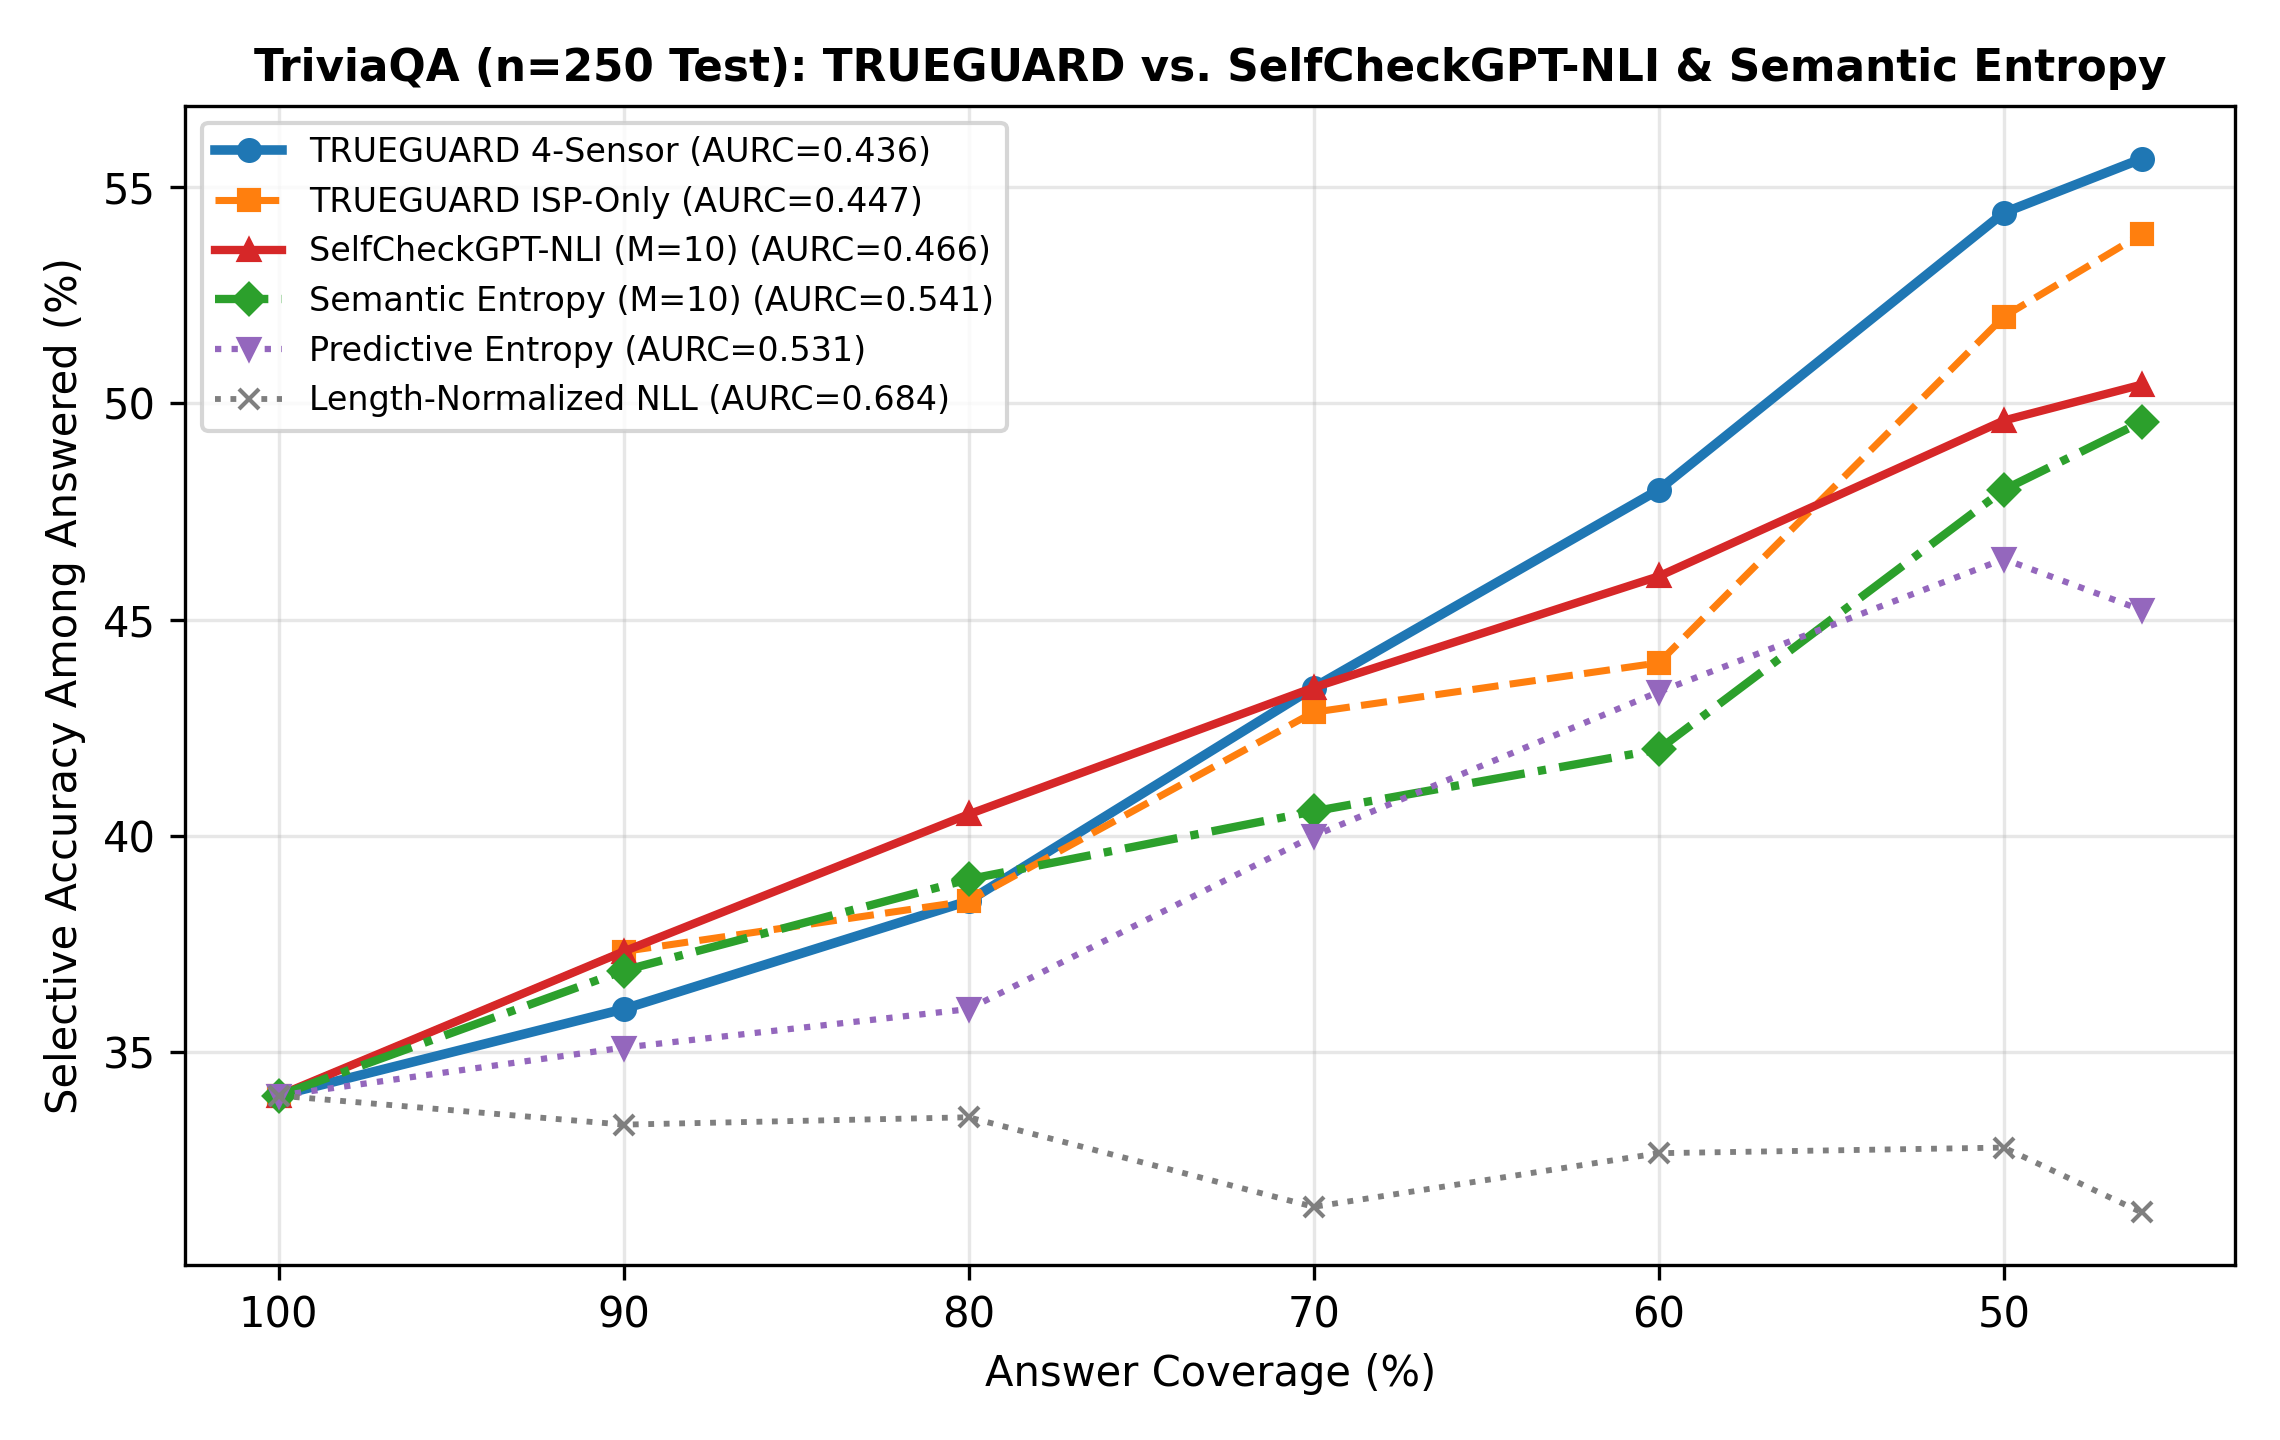
\includegraphics[width=\columnwidth]{figures/Fig7_External_Baselines_RiskCurve.png}
\caption{Risk-coverage selective prediction curves on 250 held-out TriviaQA questions comparing target-refitted TRUEGUARD with label-free SelfCheckGPT-NLI, Semantic Entropy, Predictive Entropy, and NLL.}
\label{fig:external}
\end{figure}

At matched 46.0\% answer coverage (Table~\ref{tab:mitigation}, Fig.~\ref{fig:triviaqa_abstain}), pure selective abstention achieves 64/115 correct (55.65\% selective accuracy, cutting system-wide errors from 66.00\% to 20.40\%), whereas the full three-tier controller (81 Safe, 23 Tier-1 Resample, 11 Tier-2 Wikipedia Retrieval, 135 Tier-3 Abstain) achieves 63/115 (54.78\%, -0.87\%), repairing four errors while turning three correct answers into errors. No measurable net benefit from active interventions was established on this test set.

\begin{table*}[!t]
\centering
\caption{TriviaQA Closed-Book Selective Abstention vs.\ Full Three-Tier Controller Intervention Ablation ($n_{\text{test}} = 250$)}
\label{tab:mitigation}
\resizebox{\textwidth}{!}{%
\begin{tabular}{llccccccc}
\toprule
System / Method & Role & AUROC & AURC [95\% CI] & Coverage & Correct / Ans. & Selective Acc. & Sys.\ Halluc. & Fixed / Broken \\
\midrule
Greedy Baseline & Unfiltered baseline & N/A & N/A & 100.0\% (250/250) & 85 / 250 & 34.00\% & 66.00\% & 0 / 0 \\
\textbf{TRUEGUARD Pure Abstain-Only} & \textbf{Primary selective abstention} & \textbf{0.7876} & \textbf{0.4360} [0.360, 0.524] & 46.0\% (115/250) & \textbf{64 / 115} & \textbf{55.65\%} & \textbf{20.40\%} & 0 / 0 \\
TRUEGUARD Full 3-Tier Controller & Intervention ablation (T1+T2+T3) & 0.7876 & Fixed pt & 46.0\% (115/250) & 63 / 115 & 54.78\% (-0.87\%) & 20.80\% & 4 fixed / 3 broken \\
TRUEGUARD ISP-Only (Abstain) & Single-sensor ablation & 0.7706 & 0.4473 [0.369, 0.532] & 46.0\% (115/250) & 62 / 115 & 53.91\% & 21.20\% & 0 / 0 \\
Scalars-Only (Abstain) & No-ISP ablation & 0.7130 & 0.4891 [0.404, 0.577] & 46.0\% (115/250) & 57 / 115 & 49.57\% & 23.20\% & 0 / 0 \\
Predictive Entropy (Abstain) & Uncertainty baseline & 0.6583 & 0.5309 [0.448, 0.617] & 46.0\% (115/250) & 52 / 115 & 45.22\% & 25.20\% & 0 / 0 \\
Length-Norm.\ NLL (Abstain) & Likelihood baseline & 0.4678 & 0.6843 [0.603, 0.760] & 46.0\% (115/250) & 36 / 115 & 31.30\% & 31.60\% & 0 / 0 \\
\bottomrule
\end{tabular}}
\end{table*}

\begin{figure}[!ht]
\centering
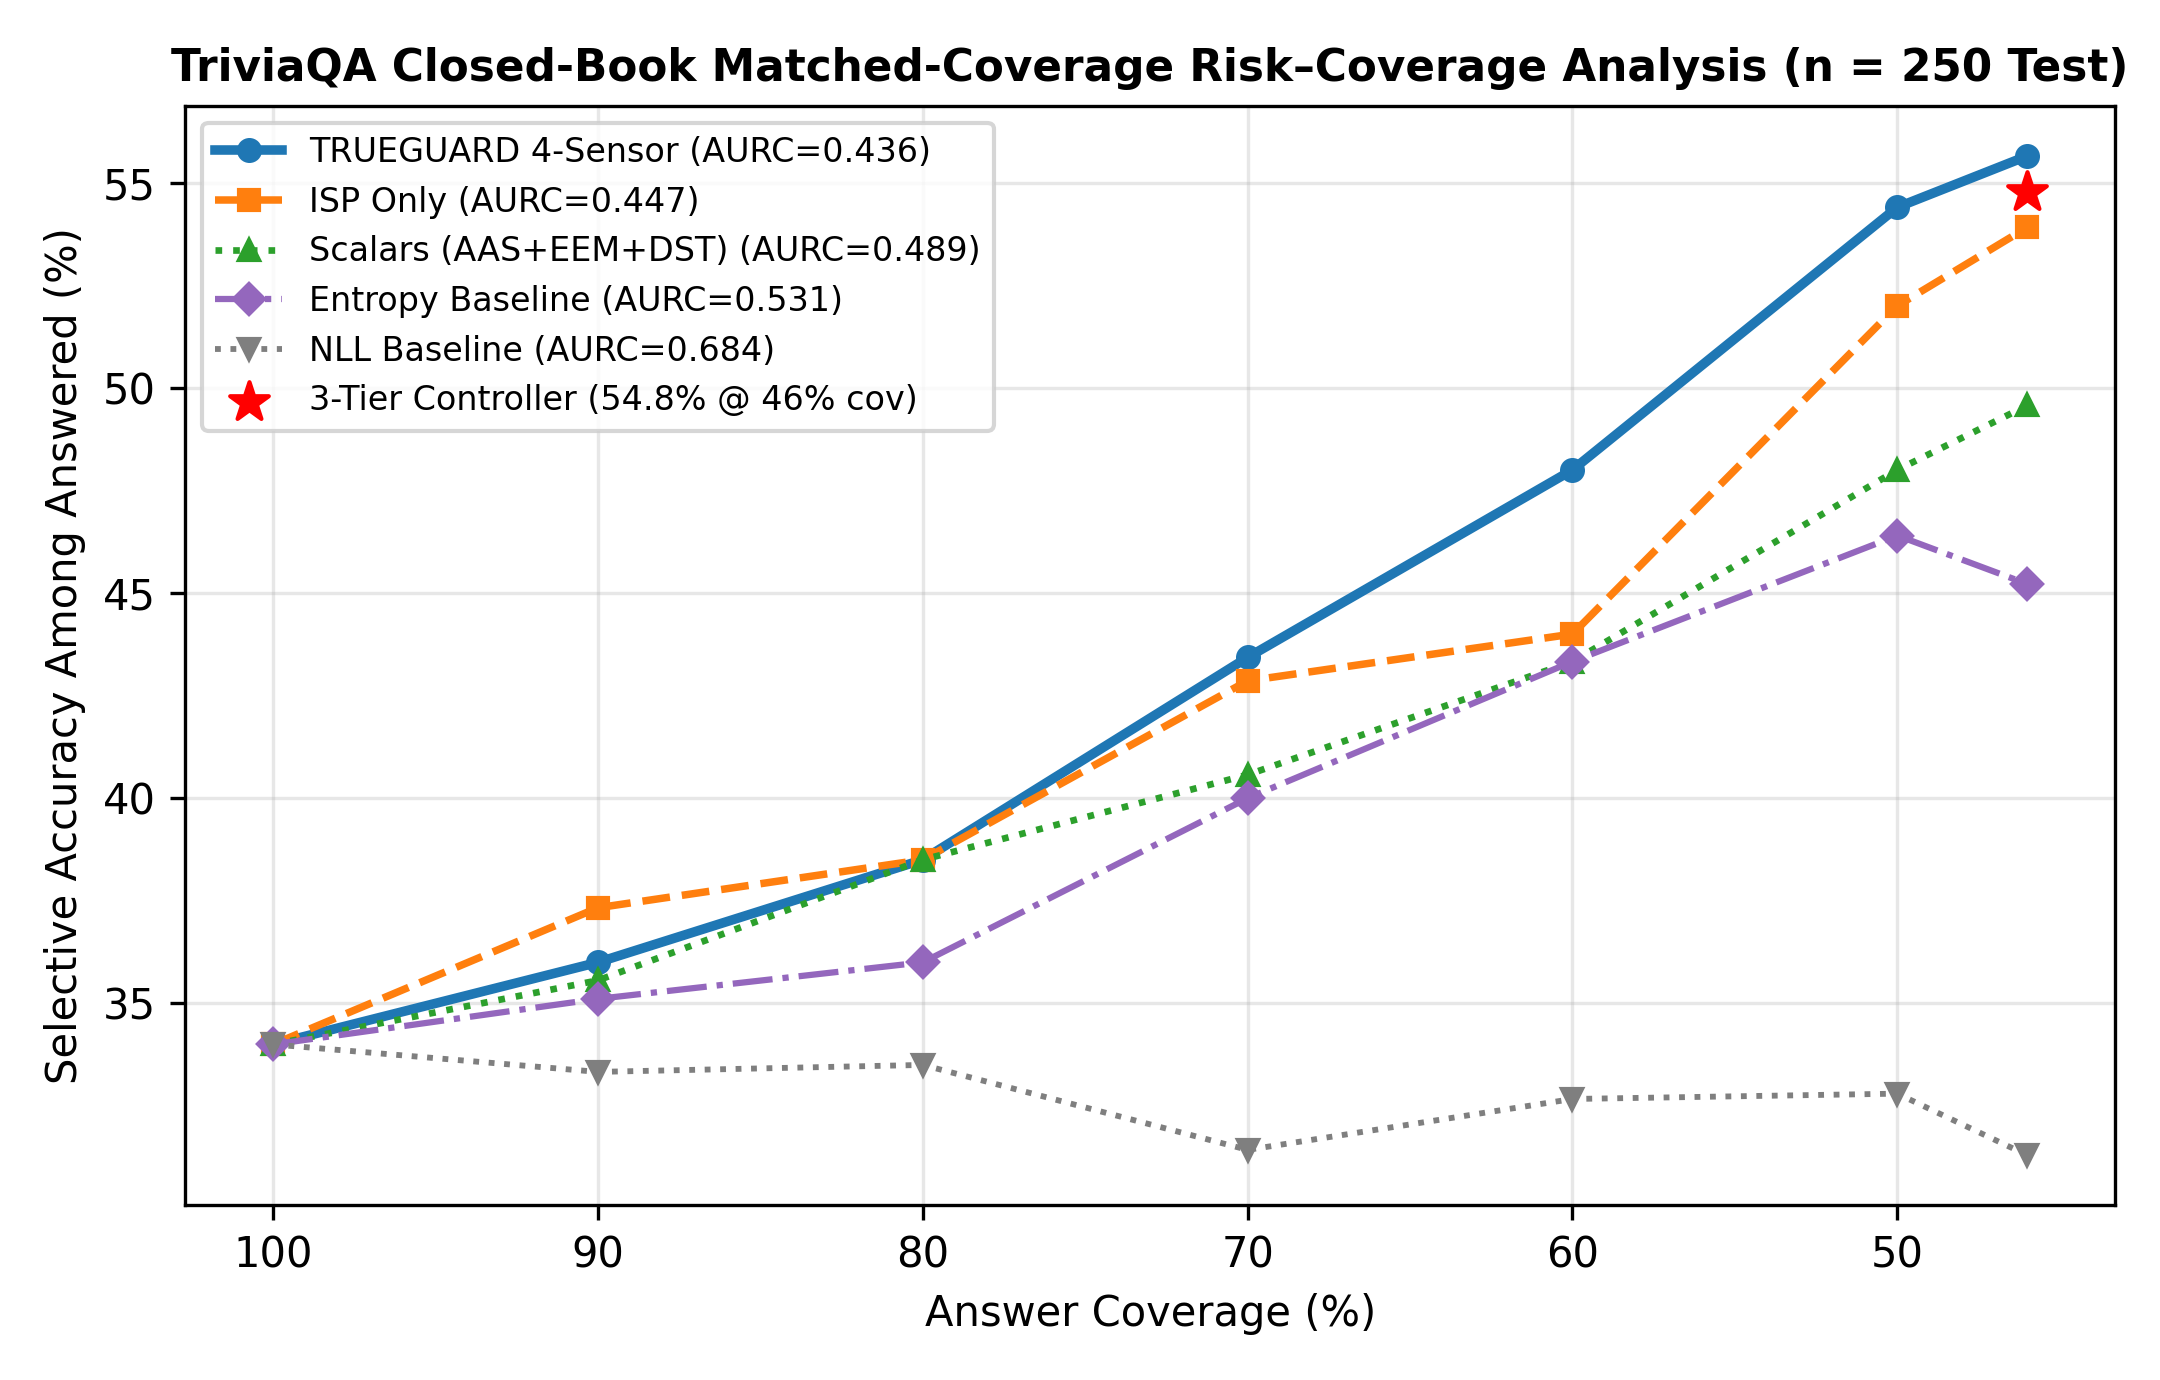
\includegraphics[width=\columnwidth]{figures/Fig3_TriviaQA_Matched_Coverage_RiskCurve.png}
\caption{Matched-coverage selective prediction accuracy on TriviaQA comparing TRUEGUARD 4-sensor fusion with ISP-only, scalars-only, predictive entropy, NLL, and the full 3-tier controller point (54.8\% at 46\% coverage).}
\label{fig:triviaqa_abstain}
\end{figure}

Under controlled sequential CUDA T4 profiling (\texttt{eager}, \texttt{bs = 1}, $25 \times 24$ tokens), vanilla TinyLlama averages 29.78~ms/token, TRUEGUARD post-pass averages 34.52~ms/token (+15.9\%, 4.60 times faster than sequential 5-sample decoding at 158.77~ms/token), and online monitoring averages 37.84~ms/token (+27.1\%, 4.20 times faster). Because the external baseline Colab run used GPU-batched \texttt{sdpa} decoding (\texttt{bs = 10}, early EOS; 0.7068~s/query SelfCheckGPT-NLI omitting the greedy pass; 1.6622~s/query Semantic Entropy with 2.47~GB NLI VRAM), our timings do not establish a wall-clock speedup over optimized batched SelfCheckGPT-NLI; TRUEGUARD's verified advantages are architectural (1 generation, 0 auxiliary 435M NLI models) and sequential.

% ==============================================================================
\section{Discussion}
\label{sec:discussion}

\subsection{Interpretation, Artifacts, and Domain Shift}
Single-pass white-box hallucination detection on a frozen 1.1B LLM depends sharply on benchmark construction, target supervision, and mitigation design. Raw HaluEval AUROCs (0.9880--0.9936) illustrate why length-matched and text-only TF-IDF controls must accompany neural metrics. Across domains, the gap between within-domain (+0.1125 to +0.6707 at $N = 900$) and cross-domain (-0.0151 to +0.0204) probe alignment is consistent with domain-dependent linear decision boundaries, aligning with both zero-shot collapse and failure of source-risk recalibration without claiming a unique causal mechanism. Because pooled fusion assigns over 96\% weight to ISP, it also suppresses length-free EEM signal on FaithDial and XSum.

\subsection{Few-Shot Refitting, Abstention, and Limitations}
Target-only refitting ($<2$~s CPU) shows clear sample-efficiency boundaries: simple baselines win at $K = 50$, while $K = 250$ delivers task-dependent gains on FaithDial, FEVER, and WikiBio yet ties 1D length on XSum. On TriviaQA, TRUEGUARD's competitive performance against SelfCheckGPT-NLI and significant gain over Semantic Entropy depend directly on 250 target calibration labels, whereas both external baselines are label-free for ranking. In this low-accuracy regime (34.00\% baseline), pure selective abstention (55.65\%) outperforms active resampling and single-passage Wikipedia retrieval (54.78\%; four fixed, three broken).

Key limitations bound our conclusions: all experiments use one frozen 1.1B model (TinyLlama-1.1B-Chat-v1.0), Datasets 1--9 use teacher-forced scoring where subtle residual artifacts may remain, TriviaQA ($n_{\text{test}} = 250$) has limited power to separate TRUEGUARD from SelfCheckGPT-NLI or ISP-only, Datasets 6--9 were inspected during zero-shot diagnosis before refitting, unsupervised white-box methods (CCS \cite{burns2023discovering}, EigenScore/INSIDE \cite{chen2024inside}) were not reproduced, and sequential latency timings are not directly comparable to GPU-batched SelfCheckGPT-NLI.

% ==============================================================================
\section{Conclusion and Future Work}
\label{sec:conclusion}

Across ten benchmarks and 32,590 evaluated sequences on frozen TinyLlama-1.1B-Chat-v1.0, our experiments support three balanced conclusions. First, raw HaluEval AUROCs are strongly inflated by length and surface style, yet white-box probing retains statistically significant gains over TF-IDF under strict length matching, dominated by ISP. Second, zero-shot pooled transfer collapses to chance across unseen domains, consistent with domain-dependent linear decision boundaries observed under equal-sample-size cosine controls, while target-only few-shot refitting ($K = 250$) yields task-dependent gains on FaithDial, FEVER, and WikiBio but matches 1D length on XSum and trails simple baselines at $K = 50$. Third, on closed-book TriviaQA, target-refitted single-pass TRUEGUARD ($K = 250$) significantly outperforms label-free Semantic Entropy and uncertainty baselines and matches SelfCheckGPT-NLI without auxiliary NLI models, while pure selective abstention (55.65\%) rather than active Tier 1/2 intervention (54.78\%) drives error reduction. Future work should replicate this artifact-controlled, supervision-aware protocol on larger open-weight models (7B--70B) and larger generation test sets ($n \ge 1{,}000$), investigate genuine cross-domain probe adaptation for $K \le 50$, benchmark reproduced unsupervised white-box baselines (CCS, EigenScore), and evaluate selective abstention alongside high-recall dense retrieval.

% ==============================================================================
\bibliographystyle{IEEEtran}
\bibliography{references}

\vspace{6pt}
\section*{Author Biographies}
\noindent\textbf{Yogesh Ravi M} is with the School of Computer Science and Engineering, Vellore Institute of Technology, Chennai, Tamil Nadu, India. His research focuses on large language model trustworthiness, hallucination detection, and selective prediction.

\vspace{4pt}
\noindent\textbf{T.\ S.\ Pradeep Kumar} (Senior Member, IEEE) is a Professor with the School of Computer Science and Engineering, Vellore Institute of Technology, Chennai, Tamil Nadu, India. He is a Senior Member of IEEE and a Senior Member of ACM.

\end{document}
